\documentclass[simplex.tex]{subfiles}
% DO NOT INCLUDE PREAMBLES/PACKAGES HERE!!
% packages are inherited from preamble.tex; you can compile this on its own
\begin{document}
\subsection{RerF}

RerF is now working in pure R code.  The running time of this
implementation is roughly the same as the Matlab implementation for
various sizes of input.  We are re-implementing portions of the code in
both C and FlashR in an attempt to reduce the running time of the
algorithm. \\


Previously, we did not have any simulation experiments in which we know
for a fact that RF is the "right" thing to do. We conducted such
experiments to see how much RerF and RR-RF lose by allowing oblique
split directions. The simulated datasets were constructed as follows.
Data was sampled in $p$ dimensions over a unit hypercube centered at the
origin. Datapoints all falling into the same orthant were assigned the
same class label. Therefore, for $p$ dimensions, there are $2^p$ unique
class labels. The true decision boundary separating the classes is
purely axis-aligned. In such a case, RF is the best classifier among the
class of all ensemble tree classifiers.

\begin{figure}[!h]
\begin{cframed}
\centering
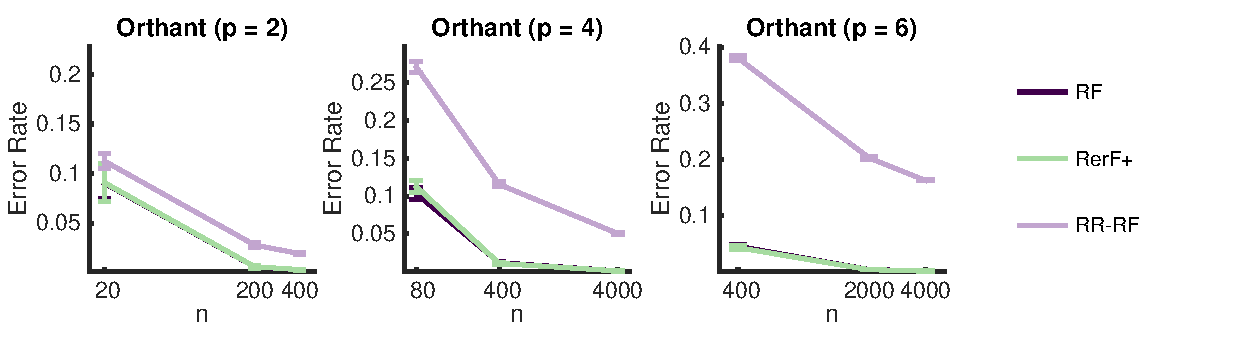
\includegraphics[width=0.85\textwidth]{../../figs/RerF.pdf}
\caption{Error rate of RF, RerF, and RR-RF on the "Orthant" dataset as a
  function of $n$, the number of training samples, for three values of
  $p$. The results indicate that there is no significant difference in
  performance between RerF and RF, while RR-RF performs significantly
  worse across all settings.}
\label{fig:name}
\end{cframed}
\end{figure}


\clearpage
\end{document}
